\subsection{Timeline}
Timestamps are used to assign an event a unique moment. With the help of these timestamps a timeline can be created. In this timeline you can see which action was done to an object at a specific time and which action followed after a specific action. In the timeline can also be represented, what kind of action (created, modified, accessed) had taken place. You can find the timestamps in different metadata of the system. Timestamps can be found on the file system metadata, application level metadata, in log data, in unallocated clusters and in other data. Metadata are data about data and are usually stored with the digital object. In different digital objects you can find different metadata. For example in a taken photo you find other metadata as in a word document. In a photo you can find information like the ISO value and exposure time which you can not find in a word document. The important metadata for the timeline are the different times. These times are called MAC times. The modified time (mtime), accessed time (atime) and changed time (ctime). It can happen that all of these times show the same time. The accessed time means the time at which the file was the last time read. The modified time means the time at which the content of the file was changed. The changed time means the time at which the metadata of a file was changed. For example a file got another permission or owner. NTFS the file system of current Windows versions owns a fourth time. This time is called born time (btime). This is the time at which the object was created. The born time is in Linux (Etx2, Ext3) not available. Appendix 1 you can see the meaning of MAC times in different file systems. In appendix 2 you see a created timeline. These timeline was created for the project and shows chronological what a criminal did. At first the criminial loaded files from the internet with illegal content. Then a truecrypt-container (setup.exe) was created and changed. Changed means in this context that to the container were probably data added. After that the criminal accessed to the data and read these data. Later, it can be seen, two other truecrypt-container were created. The data we got with the help of the tool “Redline”. Using a timeline can be reconstructed in what order the offender went on and on which objects were created, accessed or modified first.\newline \newline There are also problems with the analysis of the timeline. The timestamps are faulty if the computer which is examined is in a different time zone. One problem which exists in windows is that it can take until one hour to update the access time after it was accessed. Furthermore criminal can change the MAC times with help of software. One of these programs which can change the time stamps is named “BulkFileChanger”. BulkFileChanger can modify the created, modified and accessed time. Thus a criminal could disorient a digital forensic. All of these issues need to be considered in order to get an accurate result. One problem more sometimes it is difficult to know if an object was accessed by a application or a person. 
\newline \newline There are important hints for a digital forensics. These hints can tell a digital forensics what happened with a file. Aus paper eins zu eins kopiert.
When Modified time is equal to Created time, the file has neither been modified nor copied from another disk location. It is suggested that the file is still intact and has not been updated.

When Modified time is before Created time, the file has been copied from one system into the same/another system or moved from one partition to another partition.

In a folder, if files’ Modified times are before Created times and the files have “very close” Created times, the files have been 3
1) copied from one system to the same or another system in a
batch or
2) moved from one partition to another partition in a batch
or
3) extracted from a compressed file.
When a large number of files with “close” accessed times are found inside the hard drive, those files are likely to be scanned by some tool, e.g. anti-virus software.
If image/video files within a folder have “close” asscessed times, and no other image files have similar Accessed times,
the concerned image/video files are likely to be accessed or opened by file previewing tool, e.g. windows explorer, as
thumbnails for previewing.

When files within a folder have “scattered” Accessed times, it is highly likely that the files are accessed individually.

In a folder, if files Modified times are equal to Created times and the files have “very close” Created (Modified) times, the files may have been downloaded in a batch from another system over the network.


\begin{figure}[tbph]
	\centering
	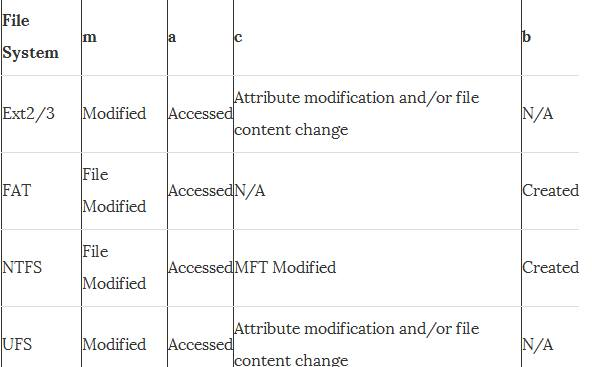
\includegraphics[width=0.7\textwidth]{graphics/mactime}
	\caption{MacTime}
	\label{fig:Mactime}
\end{figure}

\begin{figure}[tbph]
\centering
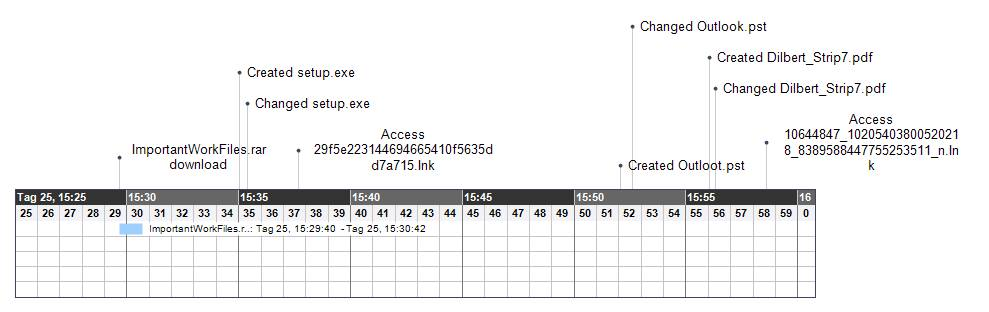
\includegraphics[width=0.7\textwidth]{graphics/timeline}
\caption{Timeline}
\label{fig:timeline}
\end{figure}
